% !TeX TS-program = 
\documentclass[12pt]{article}
\usepackage{cite} 
\usepackage{graphicx}
\usepackage{wrapfig}
\usepackage{subfigure}
\usepackage{multirow}
\usepackage{hyperref}
\usepackage{amsmath}
\usepackage{amssymb}
%\usepackage{ngerman}
\usepackage[ansinew]{inputenc}
\usepackage[left=3cm,top=3cm,bottom=3cm]{geometry}
%,right=2cm,bottom=2cm
%\renewcommand{\familydefault}{\sfdefault}

% vector graphics test
\usepackage{color}
\usepackage{transparent}
\graphicspath{{graphs/}}
\usepackage{epstopdf}
\usepackage{enumitem}
\usepackage{fancyhdr}
\setlength{\parindent}{0pt}


%\usepackage{aastex62}

%\epstopdfsetup{outdir=./}


% Abbreviations
\usepackage{acronym}

\hypersetup{
	colorlinks=true,
	linkcolor=black,
%	citecolor=black,
}
\renewcommand{\baselinestretch}{1.3}

%\setlength{\intextsep}{12pt plus 2.0pt minus 2.0pt}


%% BEGIN OF THE ACTUAL DOCUMENT %%

\begin{document}
	
%\let\jnl@style=\rm
%\def\ref@jnl#1{{\jnl@style#1}}

	
	
	\pagestyle{empty}
	\pagenumbering{roman}
	%\textasciitilde

\title{Constructing the Equation of State for Compact Stars}
\author{Jan R\"{o}der}
\date{\today}

\begin{titlepage}
    \centering
	\huge{Constructing the Equation of State for Compact Stars}\\
	\bigskip
    \large{Bachelor thesis}\\
    \huge{Jan R\"{o}der}
\end{titlepage}

%headline!!!

\makeatletter
\let\thetitle\@title
\let\theauthor\@author
\let\thedate\@date
\makeatother

\pagestyle{fancy}
\fancyhf{}
\rhead{\theauthor}
\lhead{\thetitle}
\cfoot{\thepage}



\tableofcontents



\section*{List of abbreviations}
\begin{acronym} [MRR]
	\acro{eos}[EOS]{equation of state}
	\acro{mrr}[MRR]{mass-radius relation}
	\acro{ode}[ODE] {ordinary differential equation}
	\acro{tov}[TOV]{Tolman-Oppenheimer-Volkoff equations}
\end{acronym}

\pagebreak
\pagenumbering{arabic}
\section{Introduction}

To this day, the nature of the \ac{eos} for neutron stars is highly debated. Previously discussed \ac*{eos} have emerged from various topics and models of physics. Each one has different parameters determining its impact on calculations. \\
For the past years, it has been common to derive an \ac*{eos} from a theory and then use it to construct a \ac{mrr}. That way, it was somewhat possible to investigate what impact the state of matter in different regions of the star has on a whole sequence. Since science lacks observational information about neutron star radii it has only been possible to put constraints on theories.\\
This method of constructing \ac*{mrr} has one major limitation: One cannot put an arbitrary number of theories into one \ac*{eos}. That would result in a problem impossible to solve, even for computers. Therefore, the motivation is to minimize the number of parameters and constraints in the future to find a model that is both solvable and preserves the highest physical relevance.\\
The approach chosen in this thesis inverts the above process. Instead of using an \ac*{eos} to calculate masses and radii, the latter now take over the role as input parameters. For compact stars up to a certain mass, the \ac*{eos} will be assumed to be known well enough. Above that mass a numerical reconstruction will take place, determining the \ac*{eos} from a \ac*{mrr}. Using the \ac*{mrr} as input leaves us with only the low-density region to impose an \ac*{eos} in; we do in fact have the possibility to model this region sufficiently well. If future measurements grant a decent number of data points on the \ac*{mrr}, an inverse algorithm has the potential to probe the highest densities in the universe. Due to the unique relation of \ac*{mrr} and \ac*{eos} this would mean a significant contribution to the investigation of high-density phase diagrams of, for example, quark matter. The enormous amount of energy needed to create matter at such densities exceeds everything possible by humanity; therefore a neutron star would be a welcome laboratory. The first instrument dedicated entirely to neutron star measurements is the NICER experiment located at the International Space Station. Measuring x-ray emissions directly from the star's surface and the rotational period, the radius can be determined with a precision of few hundred meters. Hopefully, a coarse \ac*{mrr} can be drawn with actual data. At that point, \ac*{eos} reconstruction will likely become a crucial part of neutron star physics.























\pagebreak
\section{Theoretical background}

\subsection{Compact stars}

At some point in a star's life, it is no longer capable of maintaining nuclear fusion in its core. Hydrogen burning first moves to a shell around the central region, further growing the previously produced helium core up to the point where helium burning ignites. Depending on the star's mass, this process can either repeat until an iron core is formed or stop at some fusion product before that. In the latter case, i.e. for star masses up to $8$\,M$_\odot$, the outer envelopes will escape the core and form a planetary nebula. What remains is a white dwarf, with an upper mass limit given by Chandrasekhar as about $1.4$\,M$_\odot$ \cite{Mazzali:2007et}. White dwarfs are the first known family of compact objects or -stars. Their interior structure depends on its progenitor star, hence their \ac*{eos} is not universally defined (\cite{Glendenning}, p. 91). Their size is of order $10^3$\,km, temperatures usually reside in the $10^4$\,K domain but can be one or two orders of magnitude higher (\cite{Glendenning}, p. 90).\\
If the fusion processes have produced an iron core, it will be compressed to densities exceeding multiple times the nuclear saturation density when the star turns into a supernova explosion. The type of remnant left behind is called neutron star, and the matter out of which it is formed is always of the same composition and state. Therefore, in contrast to white dwarfs, there is one unique \ac*{eos} to describe all neutron stars. \\
Both kinds of compact stars are subject to fast neutrino and photon cooling. After at most a few million years temperatures will have dropped several orders of magnitude below $1$\,MeV, so that on the nuclear scale the star can be  treated as cold. 



\subsection{The Tolman-Oppenheimer-Volkoff equations} \label{TOV}

The structure of compact stars will be determined by the \ac{tov}. To make analytical and numerical calculations easier, the unit system is chosen to be $c=G=1$, so that every unit is a power of length.\\
The derivation is based off the assumption that the star matter can be described as a perfect/ideal fluid. Further, the space-time shall not evolve in time, therefore staying spherically symmetric (i.e. it is stationary). In terms of the energy-momentum tensor we are left with:
\begin{equation}\label{eq:hydro}
	T_{\mu\nu}=\left(\varepsilon + P\right)u_\nu u_\mu-Pg_{\mu\nu}
\end{equation}
Where $\varepsilon$ is the energy density, $P$ is the pressure and $u_\mu$ is the 4-velocity. \\
Spherical symmetry leads to a certain form of the metric,
\begin{equation} \label{eq:line_element}
	ds^2 = e^{2\varPhi} dt^2 - e^{2\lambda}dr^2 - r^2(d\theta^2+\sin^2d\phi^2)
\end{equation}
containing spherical coordinates $r, \theta, \phi$ and a time-like coordinate $t$. Equation \ref{eq:line_element} becomes the line element for a flat space-time if the exponents in the first two coefficients become zero, from which follows the role of the exponent terms as curvature description in the radial and the time ``directions''. To be precise, $\varPhi$ is directly related to gravitational redshift, and $\lambda$ determines the change of proper length due to curvature.\\
This gives us the stress-energy tensor components:
\begin{equation}
	T_{\mu\nu} = diag(\varepsilon e^{2\varPhi}  , \ P e^{2\lambda},\ Pr^2,\ Pr^2sin^2(\theta))
\end{equation}
One now imposes conservation of energy and momentum, 
\begin{equation}
	\nabla_\nu T^{\mu\nu}=0
\end{equation}
and puts it into the Einstein equations \ref{eq:einstein} together with the metric, the components of which can be read from \ref{eq:line_element}.
\begin{equation} \label{eq:einstein}
	R_{\mu\nu} - \frac{1}{2} g_{\mu\nu} R = 8\pi \,T_{\mu\nu}
\end{equation}
Here, $R_{\mu\nu}$ is the Ricci tensor and $R$ is the Ricci scalar. Both can be calculated from the metric $g_{\mu\nu}$. Before one can get to work to get the actual \ac{tov} equations, the metric exponential functions have to be calculated.\\
One obtains, finally, the full \ac*{tov} equation:
\begin{equation}\label{eq:tov}
	\frac{dP}{dr} = \frac{(\varepsilon + P)(m + 4\pi r^3 P)}{2mr-r^2}
\end{equation}
Together with a second equation for the mass:
\begin{equation}\label{eq:mr}
	\frac{dm}{dr} = 4\pi r^2\varepsilon
\end{equation}


\subsection{The equation of state and neutron star structure} \label{eos_and_struct}

Most generally, an \ac*{eos} determines the relation between a set of quantities that future dynamics of a system can be extrapolated with. Such a set is often referred to as ``state variables''. Independent of the model applied to a certain type of matter, an \ac*{eos} takes the form
\begin{equation*}\label{eq:gen_eos}
	f(p,V,T)=0
\end{equation*}
with, in this case, pressure $p$, Volume $V$ and Temperature $T$. The nature of $f$ (the actual \ac*{eos}) is then derived from a model (e.g. nuclear or quark) to properly describe the state of matter at hand, be it a fluid, solid or of an exotic type. Here, starting on the outside of a neutron star, states are still in or not far from the range of what can be experimentally observed. Towards the inner regions, exotic states and their impact on the \ac*{eos} are still subject to investigation. A number of nuclear or fluid \ac*{eos} have been proposed, each including different aspects like interactions and states of matter, however it remains unclear how exactly a neutron star is built up. While a single \ac*{eos} for the whole neutron star would be of great interest, one usually determines the \ac*{eos} piecewise for each density region separately, imposing a phase transition between the layers. For a brief collection of models, see \cite{Pandharipande1976}.\\
The lack of information from direct measurement doesn't particularly improve this situation. However, for the first time, it might be possible to deduce information about the interior of a neutron star through data obtained by the NICER experiment located at ISS.\\
Generally, a neutron star can be divided into four zones: The inner and outer core, with inner and outer crust above it. These zones have fundamentally different properties. These zones are usually defined through their range of densities. For example, (one finds the original version of this proposal in \cite{Pandharipande1976} and \cite{ShapiroTeukolsky}), with $[\rho] =$\,g/cm$^3$:
\paragraph{$\rho\leq 10^6$} The \textit{surface} is the outermost region of the star, therefore temperature and magnetic fields can have big impact on the equation of state here. The surface may partly consist of accreted matter of unknown composition, followed by a layer of iron that marks the beginning of the actual neutron star. In this region, the \ac*{eos} is well approximated by Baym et al. \cite{Baym1971} (BPS). BPS bases calculations on a lattice configuration of nuclei as expected from a lower-density domain. This leads to significant error with respect to the ground state neutron numbers of neutron-rich nuclei further below the surface, as their masses could not be measured with sufficient precision at the time \cite{Baym1971} \cite{NeutronStars1}. 
\paragraph{$10^6 \leq \rho \leq 4.3\cdot 10^{11}$} Descending into the \textit{outer crust} a Coulomb lattice forms within a relativistic electron gas. Due to charge neutrality, $n_{electrons} = Z \cdot n_{nuclei}$; for the pressure holds $P = P_e + P_L$ \cite{NeutronStars1}, where $P_L$ resembles a correction made to account for Coulomb interactions. Upon reaching higher densities, neutronization becomes energetically favorable. In order to determine the nucleus contribution to the energy of one Wigner-Seitz cell in the lattice, BPS subtracting electron rest energies from the atomic masses. The difference between BPS and Haensel et al. \cite{HaenselPichon1994} [HP] is the model for electron screening effects. BPS used the electron binding energies as such a model, while HP subtracted those as well and imposed electron density uniformities \cite{NeutronStars1} instead.
\paragraph{$4.3\cdot 10^{11} \leq \rho \leq (2-2.4)\cdot 10^{14}$} In the \textit{inner crust} neutron-rich nuclei from a lattice; as the densities increases, neutron drip takes place. Now, there is not only an electron gas, but also a superfluid neutron gas formed by the dripped-out neutrons. A density estimate for the drip to start is performed in \cite{NeutronStars1} starting from
\begin{equation*}
	E_N(A,Z)/A\simeq E_0 + S_0 \delta^2
\end{equation*}
which is a heavily simplified nuclear mass formula. Terms were neglected until only the symmetry energy $S_0$ and the energy per nucleon in a symmetric system $E_0$ are left. $\delta=(N-Z)/A$ is also a remnant from the mass formula. At neutron drip, $\mu_n = E_0 + (2\delta + \delta^2)S_0 = 0$ and therefore $\delta_\text{ND} = \sqrt{1-(E_0/S_0)}-1$. From the beta equilibrium condition and an estimate for the electron chemical potential the drip density is about $\rho_\text{ND}\simeq 2.2\cdot 10^{11}$\,g/cm$^3$. \\
As for the \ac*{eos}, at roughly neutron drip density it is dominated by strong nucleon-nucleon interactions. There are various types of calculations and models for such a many-body system; for example, in \cite{DouchinHaensel2001} Douchin and Haensel use the Skyrme-Lyon [SLy] forces within a liquid drop model for nucleons. Likely, in this bottom region of the crust, nuclei are shaped differently to minimize their surface energy. This was first proposed by Ravenhall et al. 1983 \cite{Ravenhall1983}, where three basic shapes were used for demonstration. In the domain of the low-density phase, the higher-density phase should form spherical bubbles that turn into rods when descending further into the star. Eventually, both phases should be mixed to equal parts, nuclear matter arranged in planes. From here the process is ``reverted''; first, rods of the first phase emerge, turning into bubbles again until only the second, high-density phase is present. This phase transition is often referred to as pasta phase due to the similarities between shapes. 
\paragraph{$(2-2.4)\cdot 10^{14} \leq \rho \leq \rho_{core}$} The \textit{outer core} or \textit{neutron fluid} does no longer consist of a lattice. Remaining charge neutral, this region  
is dominated by a neutron superfluid along with a proton superfluid. The charge of the latter is evened out by electrons. In the above discussed liquid drop/SLy model, the crust-core transition appears in the \ac*{eos} as a (weak) first-order phase transition. The jump in density is in the range $1\%$.\\
The ground state of nuclear matter can be calculated from the nuclear Hamiltonian \cite{NeutronStars1}. The \ac*{eos} is determined a little easier; starting from total energy density together with conditions for fixed baryon density and electrical neutrality, Lagrange multipliers give the equilibrium conditions for the chemical potentials. For neutrinos these can be set to zero as they escape the star. Evaluating the first law of thermodynamics at equilibrium leads to the pressure. This calculation can be extended to account for particle fractions varying with density.
\paragraph{$\rho \geq \rho_{core}$} Within the \textit{inner core} lies the biggest mystery. One has no observational information about what processes happen at densities exceeding $10^{15}$\,g/cm$^3$. There are various theories about the state of matter in this region; possible are quark core formation or other types of phase transition. As a simple model, $npe\mu$ matter can be extended with a hyperon fraction. This would soften the \ac*{eos} due to a pressure drop. High-energy neutrons can convert to hyperons, resulting in a lower energy state (which contributes to the pressure) but a higher mass \cite{NeutronStars1}. 


% Stiffness of EOS
% Dependence of R on M


\subsection{General constraints}

%There are two major conditions for any equation of state to be physically acceptable. For one, it cannot be \textit{ultrabaric}, i.e. $P>\epsilon$. Sometimes this is confused with the causality limit. An EOS might be ultrabaric and still causal: the condition reads $dP/d\epsilon=(v/c_s)^2 < 1$ with effective sound speed $c_s$. However, if the EOS starts below the ultrabaric line and fulfills the causality condition, it will never cross that line. If its slope increases so that $dP/d\epsilon>1$, the EOS becomes \textit{superluminal}. While a superluminal EOS is widely thought to be acausal, that is not necessarily the case. In general neither Lorentz invariance nor causality explicitly forbid $v>c_s$ \cite{NeutronStars1}, but such EOS all have other significant disadvantages leaving them irrelevant. 



There are two major conditions for any equation of state to be physically acceptable. For one, it cannot be \textit{ultrabaric}, i.e. $P>\epsilon$. Sometimes this is confused with the superluminal limit even though an \ac*{eos} might be ultrabaric and still subluminal. A physically relevant \ac*{eos} cannot be superluminal either, the condition reads $dP/d\epsilon=(v/c_s)^2 < 1$ with effective sound speed $c_s$. The confusion of the two terms arises because an \ac*{eos} starts fulfilling both conditions, it will never cross the ultrabaric line. If its slope increases so that $dP/d\epsilon>1$, the \ac*{eos} becomes \textit{superluminal}. While a superluminal \ac*{eos} is widely thought to be acausal, that is not necessarily the case. In general neither Lorentz invariance nor causality explicitly forbid $v>c_s$ \cite{NeutronStars1}, but such \ac*{eos} all have other significant disadvantages leaving them irrelevant. 

\subsection{Stability, mass-radius relation and third family}

The term \textit{stability} is generally used in the context of stability towards perturbations, i.e. radial oscillation modes. This can be read off the mass-radius relation: If the curve reaches a critical point, the slope changes sign and the lowest stable mode switches its stability. Reading from the right, a counter-clockwise change of slope at a critical point leads to instability of a mode. This can be seen in \ref{fig:third_stable}.
\begin{figure} [h]
	\centering
	\bigskip
	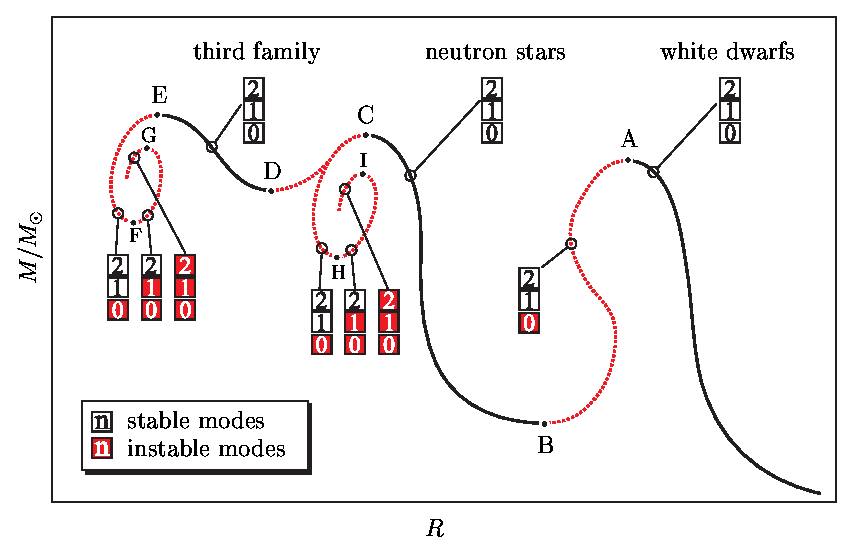
\includegraphics[width=0.9\textwidth]{graphs_pdf/third_and_stable}
	\caption{Mass-radius relation with a third stable branch and stability of lowest modes. Taken from \cite{Schertler2000}.}
	\bigskip
	\label{fig:third_stable}
\end{figure}
At points A, C and E, the maximum masses and minimum radii for one family each, the fundamental mode becomes unstable ($n=0$). $n$ is the number of radial nodes. When a new family starts with its lowest mass, $n=0$ regains stability. A branch is required to have all modes stable against oscillation to be physically relevant as a family. \\
A branch usually ends when the \ac*{eos} becomes sufficiently soft. A phase transition can then lead to a sudden increase in slope, causing the \ac*{mrr} to rise again, to a new branch. For example, a white dwarf is stabilized by the Pauli principle; if it crosses a certain mass limit, it collapses to a neutron star until strong interaction and degeneracy block further compactification. In \ref{fig:third_stable} the neutron star branch hosts mixed phase cores, i.e. nuclear along with quark matter. Their high-mass twins (more below) do have a mixed phase region, but their core consists of pure quark matter. The interior structure is heavily influenced by the \ac*{eos} for all three regions, while the hadronic phase \ac*{eos} is assumed to be known relatively well. \\
In 1966 Wheeler showed that, if the \ac*{eos} was smooth, there would only remain a white dwarf and a neutron star branch in the \ac*{mrr} that would contain stable configurations. However, in 2000 Glendenning and Kettner discovered a class of \ac*{eos} that in contrast to Wheeler's work produced a third stable branch in the \ac*{mrr} \cite{GlennKett}. These stars would have the same masses as neutron stars (depending on the exact \ac*{eos}, this might hold for a certain mass window) but significantly smaller radii. Therefore, these stars are generally referred to as "high mass twins" or "twin stars". \\
The main arguments against a third family would be instability to oscillations (resulting in explosion oder black hole formation) and distribution of Fermi pressure among more flavors \cite{GlennKett}. Most theories resolve around quark core formation and a pasta-like phase transition from hadronic/mixed phase to quark matter analogue to the zone between crust and core. \\
The first to discover the general possibility of a third family was Gerlach in 1968 \cite{Gerlach1968}; in the process of investigating his theory that some kind of sub-nuclear density interaction may have a significant impact on the \ac*{eos} and \ac*{mrr} he was also the first to explore an inverse approach to stellar structure calculation. For more on that, see \ref{inv}.

\subsection{Yet another compact family?}

In 2017 M. Alford and A. Sedrakian were the first to argue what effects a multiple phase QCD diagram would yield for new families of compact stars (\cite{AlfordSedrakian2017} and references therein). Up to that point a quark core was always assumed to consist of only one phase. \\ 
In order to construct an \ac*{mrr} Alford and Sedrakian put together a piecewise \ac*{eos} consisting of one for nuclear (hadronic) matter up to saturation density and one for above densities. The latter part is allowed to have two first-order phase transitions, with a constant speed of sound per quark phase. The \ac*{eos} then looks as follows:
\begin{figure} [h]
	\bigskip
	\centering
	\subfigure[Constructed \ac*{eos}]{\includegraphics[width=0.46\textwidth]{graphs_pdf/EoS_letter}} 
	\subfigure[Corresponding \ac*{mrr}]{\includegraphics[width=0.5\textwidth]{graphs_pdf/mass_radius_stiff2SC}}
	\caption{(a) Constructed \ac*{eos} for a second quark matter phase transition. (b) \ac*{mrr} corresponding to stiff two-flavor color superconducting [2CS] and color-flavor-locked [CFL]. Taken from \cite{AlfordSedrakian2017}.}
	\bigskip
	\label{fig:fourth_eos_alfsed}
\end{figure}
From figure \ref{fig:fourth_eos_alfsed} a) four of the six parameters determining the \ac*{eos} can be read off: the transition pressures $P_{1,2}$ as well as $\Delta\varepsilon_{1,2}$, the energy density jumps. The remaining parameters are the phases' sound speeds. Figure \ref{fig:fourth_eos_alfsed} b) shows an \ac*{mrr} for four different energy density jump ratios and stiff quark phase \ac*{eos}. The sound speeds $s_1$ and $s_2$ have been set to 0.7 and 1, respectively. For jump ratios above of about 0.15, a fourth branch of compact stars separates from the twin stars located around 12.5\,km. White dwarfs are not shown, the very right branch is made of neutron stars. Within a certain ratio range triplet configurations arise: one mass, but three possible radii, depending on the star's composition. This is well visualized in fig. \ref{fig:composition}. If the phase transitions are sufficiently weakly first order, no instability arises, leaving the \ac*{mrr} with an extended twin star branch. From there, the fourth family emerges, completely vanishing when both transitions are strong enough, making both quark phases unstable.
\begin{figure} [h]
	\centering
	\includegraphics[width=0.9\textwidth]{graphs_pdf/profiles}
	\caption{States of matter for a triplet configuration. $M=1.975$\,$M_\odot$, $\Delta\varepsilon_{1}/\Delta\varepsilon_{2}=0.23$. Pressure in dyn/cm$^2$, N stands for Nuclear Phase. Taken from \cite{AlfordSedrakian2017}.}
	\label{fig:composition}
\end{figure}



\subsection{Fermi gas equation of state}

This \ac*{eos} will serve as a test case for the reconstruction algorithm (the constant in the polytrope will be set arbitrarily when using it as a first test). For a detailed version of this derivation, see \cite{Glendenning}. \\
Here, $p=k$ ($c=1$) and therefore $E=\sqrt{k^2+m^2}$. With that, the energy density, pressure and density become:
\begin{align}
	\varepsilon &= \frac{\gamma}{2\pi ^2}\int_{0}^{k_F} k^2\sqrt{k^2+m^2} \ dk \\
	p &=  \frac{\gamma}{6\pi ^2} \int_{0}^{k_F} \frac{k^4}{\sqrt{k^2+m^2}} \ dk \\
	\rho &= \frac{\gamma}{2\pi ^2}\int_{0}^{k_F} k^2 \ dk
\end{align}
Setting the chemical potential to $\mu = \sqrt{k_F^2+m^2}$ (the Fermi energy), the solutions to these integrals read
\begin{align} \label{eq:eorho_solved}
	\varepsilon &= \frac{1}{4\pi^2} \left[  \mu k_F \left(\mu^2-\frac{m^2}{2}\right)-\frac{m^4}{2} \ln \left(\frac{\mu +k_F}{m}\right)   \right] \\
	p &= \frac{1}{12\pi^2} \left[  \mu k_F \left(\mu^2-\frac{5m^2}{2}\right)-\frac{3m^4}{2} \ln \left(\frac{\mu +k_F}{m}\right)   \right] \\
	\rho &= \frac{k_F^3}{3\pi^2} \label{eq:rho}
\end{align}
where $\gamma = 2$, the degeneracy factor for fermions due to spin orientation. The Pauli principle is therefore directly included. Charge neutrality can be imposed, and chemical equilibrium can be obtained as
\begin{equation}
	\mu_n = \mu_p + \mu_e
\end{equation}
with chemical potentials for neutrons, protons and electrons.\\
Numerically, it is convenient to calculate limits of equations \ref{eq:eorho_solved} - \ref{eq:rho} for the case of high and low densities, i. e. $k_F \gg m$ or $k_F \ll m$. Our test case \ac*{eos} will resemble very low densities. Expanding \ref{eq:eorho_solved} in $k_F/m$ one obtains
\begin{equation}
	p\sim K\cdot \rho^{5/3}
\end{equation}
Which is a polytropic type of equation. By absorbing densities into the energy density, one can get
\begin{equation}
	p = K\cdot\varepsilon^\gamma
\end{equation}
which is common to use for simple star models, especially white dwarfs. 


\subsection{Numerical solution}

The TOV equations come in the form of a first-order \ac{ode} system. In order to obtain sufficient precision, a 4th-order Runge-Kutta algorithm can be used to solve said \ac{ode}. By looking at both equations, our \ac{ode} system is given in the form:
\begin{equation}\label{eq:ode}
	\dot{y}(t) = f(y(t), t)
\end{equation}
where $\dot{y}(t)$ is a two component "vector":
\begin{equation}
	\dot{y}(t) =  \left( \begin{array}{c}dP/dr\\dm/dr\end{array} \right)
\end{equation}
$f(y(t), t)$ then contains the right hand side of equations \ref{eq:tov} and \ref{eq:mr}. \\
Numerically, solving the ODE is achieved by approximation of a step $\tau$ in the function variable $t$ (in \ac{tov}, this is the radius $r$) with derivatives of the function that is the ODE solution ($y$). 
\begin{equation}
	y(t+\tau) = y(t) + \frac{1}{6} (k_1 + 2k_2 + 2k_3 + k_4)
 \end{equation}
with increments $k_i$:
\begin{align*}
	k_1 &= f(y(t),t)\cdot\tau\\
	k_2 &= f(y(t)+k_1/2,t+\tau/2)\cdot\tau\\
	k_3 &= f(y(t)+k_2/2,t+\tau/2)\cdot\tau\\
	k_4 &= f(y(t)+k_3,t+\tau)\cdot\tau
\end{align*}
All $k_i$ are of course also two component "vectors". \\
For simpler test versions of the code, it is convenient to reduce the RK4 algorithm to RK1, or Euler's method. Also, the step size does not have to be adaptive. That way, runtime efficiency can be adjusted.

\subsubsection{Adaptive step size}

If mass and radius calculation algorithms do not yield a sufficient precision, the step size within the \ac*{tov} solver can be implemented as an adaptive variable instead of a constant. Step size adaption works as follows: In order to maintain a minimum level of precision, the program checks for the change in pressure resulting from one Runge-Kutta step. If this change is too large, the step size $\tau$ is varied by a factor and the Runge-Kutta step count is reduced by one. Upon repeating the step, the same check takes place, and if necessary another $\tau$ is adjusted again. If the check is successful, the program will accept the step result and proceed with the next one. 

\subsubsection{Implementation}

In the actual program (written in C), the left hand side of our \ac{ode} system is implemented as a two-dimensional array of form y[N][x]. N will be two, for the whole program, as we will not add other equations to the system. $k_i$ are all one-dimensional arrays; that way $x$ is only reflecting the step count. $x$ will therefore be in range zero up to the number of iteration steps. We set an arbitrary maximum step amount to prevent segmentation faults. The RK4 algorithm will be implemented easily modifiable at any time to another order of Runge-Kutta or even Euler.


\subsection{From TOV solver to reconstruction}

After implementing the \ac{tov} equations together with the integration method, one can now generate an \ac*{mrr} by looping over several central pressures using one \ac*{eos} only. This \ac*{mrr} will be used for testing the final reconstruction code, which will consist of the \ac{tov} solver extended with the reconstruction algorithm explained below.\\
The main additions will be the splitting of the pressure range into segments, each requiring their own part of the \ac*{eos}, as well as a segment determining the ``correctness'' of calculated mass and radius. The code will work not as ``inversely'' as proposed below; the stars will still be integrated from the core towards the surface. However, the reconstruction no longer uses one single \ac*{eos} but rather constructs its own.


\subsection{The inverse problem} \label{inv}
The ``standard'' problem of stellar structure is an integration of the TOV equations with a given \ac*{eos} and central pressure, determining the total mass and radius (values of the variables at the surface). 
The inversion of this ``standard'' problem was originally brought up by Gerlach in 1968, in a paper investigating the possibility of a third stable family \cite{Gerlach1968}. Another well-established method was developed by Lindblom. Both methods shall be recalled here.\\
Just like any other published approach to the problem, Gerlach assumes the \ac*{eos} to be known below a certain density. In order to determine the changes in density and mass for the core region of unknown type for the next configuration, he sets up variations for the \ac{tov} equation \ref{eq:tov}:
\begin{align}
	\frac{d\Delta\rho}{dr} &= A(r) \Delta\rho + B\Delta m \\
	\frac{d\Delta m}{dr} &= 4\pi r^2\Delta \rho
\end{align}
Note that Gerlach used $\rho$ instead of $\epsilon$ in his equations. From here he solves the inverse problem in two steps. First, he requires the changes made to a star's surface in terms of radius and mass to be related to changes at the beginning of the core region, here in terms of density and mass. Next, he specifically calculates $\Delta \rho$ and $\Delta m$ for the core, which are required to smoothly fit to the core surface. Gerlach puts the above equations in matrix form and includes an iterative method, together with proper matching conditions. \\
Lindblom on the other hand presents an \ac*{mrr}-\ac*{eos}-pair to be uniquely linked by an abstract map \cite{Lindblom1992}. This gives rise to the possibility of using that map in the other direction, i.e. from \ac*{mrr} to \ac*{eos}. His ``traditional'' solution of the inverse problem works as follows:\\
Instead of integrating the \ac{tov} equations from the core towards the surface with initial values $p=p_c$ and $r=0$, Lindblom uses $M=m(R_{surface})=m(R)$ and $R$ as starting point to the calculation. Also, the \ac*{eos} is assumed to be known up to some pair \{$\epsilon_i, p_i$\} corresponding to a star \{$M_i, R_i$\} (as Gerlach did). Looking at the next star, \{$M_{i+1}, R_{i+1}$\} are set as initial values and integration takes place until \{$\epsilon, p$\} reach \{$\epsilon_i, p_i$\}. At this point, a core \{$m_{i+1}, r_{i+1}$\} is left to be integrated. Expanding the TOV equations in this small region as a power series and inverting that, \{$\epsilon_{i+1}, p_{i+1}$\} can be obtained as a function of previously calculated quantities. This process is repeated for the rest of the \ac*{mrr}, linking \{$\epsilon_{i+1}, p_{i+1}$\} to the known \ac*{eos} by interpolation.\\
Here, a different and more simplistic approach to this problem is developed. This new method does not require the star to be integrated from crust to core, but will merely be a modification of the standard problem. This leads to a kind of ``trial and error'' type of solution, as section \ref{recon_method_sec} will explain more detailed.

\pagebreak
\section{Reconstruction method} \label{recon_method_sec}

\subsection{General goal}

The goal is to reconstruct the \ac*{eos} with as few biasing and imposing of mathematical form as possible. Therefore, the only pre-determined input is an \ac*{eos} corresponding to a given mass in the \ac*{mrr} (Fig. \ref{fig:mce}). From there, the \ac*{eos} can be constructed without further constraint. Here, a straight line is added to the end of the \ac*{eos}, that is, in the high density region (Fig. \ref{fig:recon} b). The ODE solver starts at a point near the end of the given \ac*{eos} and will calculate a mass with the (now small) piece of straight line and the \ac*{eos}. If the mass does not fit the corresponding one in the \ac*{mrr} that was read in previously, the starting point on the line will be shifted to a higher pressure by a small step. At some very high pressure, a cut-off can be applied due to un-physical energy densities. If the starting point reaches the cut-off and the correct mass was not found, the slope of the line is varied. The latter also happens when the radius that corresponds to the calculated mass does not fit the one corresponding to the radius in the file. in Fig. \ref{fig:recon} c) the slope and end point of the green line have been successfully varied and the next mass and radius are reconstructed using the variation of the red line. The green line is now a part of the given \ac*{eos}. This process will be repeated until the end of the \ac*{mrr} file.
\begin{figure} [h]
	\centering
	\bigskip
	\includegraphics[width=0.9\textwidth]{graphs_pdf/mrr_corr_eos_new}
	\caption{corresponding points in \ac*{mrr} and \ac*{eos}. Point in \ac*{eos} resembles values in the center of the star.}
	\bigskip
	\label{fig:mce}
\end{figure}
\begin{figure} [h]
	\centering
	\bigskip
	\includegraphics[width=1\textwidth]{graphs_pdf/eos_lines_recon_schematic}
	\caption{a) Given polytropic equation of state, b) added a constructed straight line, c) Successfully varied green line, red line for next mass}
	\bigskip
	\label{fig:recon}
\end{figure}


\subsection{Pressure intervals}

For the first mass in the file that is supposed to be reconstructed, the code will use the given \ac*{eos} over the complete pressure interval $p_c$ to 0. That way, the first mass can be reproduced exactly in a test case. $p_c$ will be the last pressure value of the given \ac*{eos} interval. From there, lines will be added to that end point; in the program, a flag labelled ``one'' will be set to false after the first mass was calculated. \\
From this point on it is important to determine which \ac*{eos} will be used for what pressure interval inside the star. The second mass to be calculated will use the given \ac*{eos} and one single line after it; masses number three and above then also need a line, but before finishing with the given \ac*{eos} the previously determined lines are supposed to fill in the rest of the pressure range. \\
The line currently subject to variation will start at the central pressure ($p_c$) and will end at the last pressure a star was reconstructed for. This is resembled by the end point of the last previous line (or in the special case, the last pressure of the given \ac*{eos}). The last given \ac*{eos} pressure is saved in the very beginning as $p_{init}$, marking the point from which the given \ac*{eos} will finish up the mass calculation.


\subsection{Linear interpolation}

Four parameters are needed to calculate one line equation (two points in a two-dimensional plane). In the code, every \ac*{eos} point consists of a pressure and an energy density value. The parameters needed for one line are stored in an array $\alpha$: 
\begin{equation*}
	\left(\alpha_0,\,\alpha_1,\,\alpha_2,\,\alpha_3\right) = \left(p_1,\,\varepsilon_{1},\,p_2,\,\varepsilon_{2}\right)
\end{equation*}
Inserting this array into $y = mx+b$ or rather $\varepsilon = mp+b$, the line equation looks as follows:
\begin{equation} \label{eq:e(p)_line}
	\varepsilon(p) = \left(p-\alpha_1\right)\frac{\alpha_3-\alpha_1}{\alpha_2-\alpha_0}+\alpha_0
\end{equation}
where $m=\Delta\varepsilon/\Delta p$ and $b$ is the y axis point.
While one line is being varied, $\alpha_0$ and $\alpha_1$ stay fixed as they are the last line's end point. Calculating the mass, $\alpha_2$ is varied at fixed $\alpha_3$. If the corresponding radius does not fit, $\alpha_3$ is shifted through a slope change. If mass and radius have been reconstructed with sufficient precision, the $\alpha$ array is extended by two in order to fit in the next end point to be varied. The \ac*{eos} function always checks which interval the current pressure lies in to determine the $\alpha$ for further calculation. The array will be extended to index values high above three; here, zero to three were chosen. In the actual program, $(\alpha_0,\alpha_1)$ resembles the known \ac*{eos} region's end. In order to generalize equation \ref{eq:e(p)_line}, in index $i$ is introduced and initialized with alpha.size()$-2$. In the above special case, alpha.size() (C function) would equal to four. The subscripts in \ref{eq:e(p)_line} are now rewritten with $i$:
\begin{equation} \label{eq:e(p)_indx}
\varepsilon(p) = \left(p-\alpha_{i-1}\right)\frac{\alpha_{i+1}-\alpha_{i-1}}{\alpha_i-\alpha_{i-2}}+\alpha_{i-2}
\end{equation}
That way, the array can be more easily accessed an used by the code even with continuous extension.\\
Centering the whole reconstruction around the $\alpha$ array also immediately makes external \ac*{eos} input possible. An \ac*{eos} table read in by the code along with an \ac*{mrr} would be stored in $\alpha$ and used for the calculation with either the same linear function as the rest, or with another interpolation method. Note that the external table would need the energy density density in one column (many \ac*{eos} use the matter or baryon density instead).

\subsection{Alternative method: Monte Carlo}

In case the previously described algorithm is not capable of finding all correct radii and masses, an alternative shall be proposed here. \\
As before, up to a certain central pressure a known \ac*{eos} will be applied. The next point will be defined as a ``box'' around a pressure some step higher that the previous one. Within that box, a Monte Carlo simulation generates energy densities and pressures, to be combined (every pressure with every energy density) to central values used for the calculation. The best point will then be the new central value and in further calculation a line will be drawn between that and the previous pressure. If this best point does not reach the wanted mass or radius, the Monte Carlo simulation will be repeated with more data points. \\
Alternatively, a Monte Carlo reconstruction would technically be capable of drawing a complete (somewhat arbitrary) \ac*{eos} and varying it as a whole. Still, the curve would be discretized, for example into bins defined by certain pressure ranges. With that curve an \ac*{mrr} could be drawn with some number of stars. The drawn curve could then be compared to the input curve as a whole, constraining some global variation parameter by using a probability method (e.g. the Metropolis algorithm). The advantage of drawing the whole \ac*{eos} is that the produced \ac*{mrr} can be of any precision (central pressure separation between stars). With the input \ac*{mrr} and an interpolation method of some kind for both \ac*{mrr} the two could be compared using for example a method of least squares, therefore discretizing both curves in the same manner. The sum of least squares would be a possible parameter for the Metropolis algorithm.\\
 That way, the mass-radius points generated by the code would not have to be the same as those in the input data. Curve comparison should indeed take place using interpolation of points as an \ac*{mrr} does not follow a type of function that could be used fit it to the data. \\
This method is of course of highly numerical nature. However, in the past statistical approaches have often been of great success, which is why here a Monte Carlo method could potentially be used as a comparison. 

\subsection{Optimal radius and mass for a given slope}

Before comparing the radius to the input, the optimum mass can easily be obtained by fixing a slope for the \ac*{eos} and varying the central pressure in small steps. The latter has no significant impact on the radius. Here it proved to be convenient to use an indirect check instead of a direct comparison to the input mass. After the first calculation, an initial difference between input and outcome is stored. The difference for the next central pressure will be multiplied with the initial one; variation takes place until the multiplication outcome flips the sign. Then, the pressure step is decreased and variation also switches direction. This can be repeated until a desired precision is reached. The radius corresponding to the optimum mass will be given to the main function along with it. 

\subsection{Direct and indirect radius check} \label{indradch}

Upon finishing the calculation for a star, the code is to check mass and radius. This can either be done by directly comparing the calculated values with the input (in the following, direct method) or by choosing an indirect way of doing so. The direct method can be described as search for the root of a function $f_\text{dir}$:
\begin{equation*} \label{eq:direct}
	f_\text{dir} = R_\text{calc}-R_\text{want}
\end{equation*}
An elegant way to unite radius and slope control is by choosing an indirect method function $f_\text{ind}$:
\begin{equation*} \label{eq:indirect}
	f_\text{ind} = \left(R_\text{calc}-R_\text{want}\right)^2 + \lambda\cdot \left(\xi_\text{curr} - \xi_\text{prev}\right)^2
\end{equation*}  
Instead of trying to find the roots of $f_\text{dir}$, the code is now supposed to find extrema of $f_\text{ind}$. The functions are loosely related as 
\begin{equation*}
	f_\text{ind} \sim \int f_\text{dir}
\end{equation*}
$\lambda$ is an ``importance parameter''. In order to avoid big jumps in the slope $\xi_\text{curr}$ with respect to $\xi_\text{prev}$, $\lambda$ is set to some value. That way, $\xi_\text{curr}$ will not deviate more from $\xi_\text{prev}$ than $\lambda$ allows. Before the variation of a slope, a star is calculated once with the current slope and with a higher and lower one, respectively. The slope variation direction is then determined by the behaviour of $f_\text{ind}$. After the first reconstruction $\lambda$ is set to a value above zero while initially using $\lambda = 0$ as there is no slope from before to use. \\
Some time in the future, the program should be capable of modelling first-order phase transitions in the \ac*{eos}. Such a transition requires a jump in the slope and discontinuities in the \ac*{eos}. It is obvious that the indirect method is biased towards smooth \ac*{eos} without any unusual progression $-$ ruling out the possibility to model a phase transition from the beginning. That can be dealt with by tracking extremal points in the \ac*{mrr} while reading it in as input. When the reconstruction part of the code reaches the first mass behind a maximum, the algorithm is changed from $f_\text{ind}$ to $f_\text{dir}$ by setting $\lambda = 0$. $\xi_\text{curr}$ may now freely deviate from $\xi_\text{prev}$ to find the \ac*{eos} points during and after the transition. \\

\pagebreak
\section{Results}

\subsection{Issues}

During development of the code, various smaller and bigger issues had to be dealt with or worked around. A rather fundamental question that is what numerical methods can or should be allowed in order to get nice and physically relevant results while still being able to motivate a numerical change with physics. For example, during some development stages cut-offs or statements were implemented that should only be taken into account by the code at a certain point through the \ac*{mrr}, which is obviously not particularly physical. The first attempt at global constraints in the calculation was the introduction of an indirect method; the $\lambda$ importance parameter was the consequence of assuming the \ac*{eos} to be (rather) smooth. Radius control issues will now be discussed in a more detailed fashion.

\subsubsection{Radius and slope control}

While the direct method \ref{eq:direct} somewhat works in the low-density region, it quickly starts suffering from big slope jumps for the reconstructed lines. Some \ac*{mrr} points are found corresponding to values above the wanted \ac*{eos} curve, continuing with only very slight changes in slope until points below the \ac*{eos} are used for calculation. From there, a slope jump pushes the next point above the curve again. These jumps get bigger and pile up to a point where the code cannot push the current energy density above the \ac*{eos} again; from here, none of the produced values are of use as now all further points strongly deviate from the \ac*{eos}.\\
Initially, the indirect method \ref{eq:indirect} was chosen to ensure that the slope would not contain big jumps. This however has a huge impact on runtime, but as efficiency was not the main goal, optimization was postponed. The biggest problem is, ironically, the precision needed to avoid slope jumps. At some point, the code will calculate in slope steps so small that radius changes start to become exceedingly rare. As discussed by various researchers, the radius does not depend on a specific parameter and often requires drastic changes in various values used in the calculation. Here, the slope is often the only parameter that would have any impact in the first place; the mass is relatively easy to find along with a rather accurate central pressure. The indirect method included the $\lambda$ parameter in order to connect a radius check with a condition regarding the slope with respect to the previous one. $\lambda$ is to determine the maximum deviation of a reconstructed point from the curve, here is however no way of determining a ``perfect'' $\lambda$ other than trial and error. The parameter remains rather arbitrary even though it can be motivated with a smoothness assumption. What that means for phase transitions has been discussed in \ref{indradch}: a transition has immediate effect on the \ac*{mrr}, the code can therefore be modified based on input analysis. When the reconstruction reaches the point of transition, $\lambda$ is used to modify the algorithm accordingly. \\
Setting $\lambda = 0$ of course bears the risk ``finding'' wrong points easily as there is less control over how the calculation deals with the extra degree of freedom. If in the rest of the reconstruction small errors appeared, the calculation will probably not find a decent radius at all. If now the constraints are loosened, precision in evaluating the dimensions and properties of the phase transitions are sacrificed.

\subsection{Test case}

The first code test will take place with a simple polytropic \ac*{eos} such as
\begin{equation*}
\varepsilon(p) = \left(\frac{p}{10}\right)^{3/5}
\end{equation*}
Using the TOV solver, an \ac*{mrr} is generated. The \ac*{mrr} seen in Fig. \ref{fig:test} will be the first one to be reconstructed. 
\begin{figure} [h]
	\centering
	\bigskip
	\includegraphics[width=1\textwidth]{graphs_pdf/testcase_mrr_eos}
	\caption{Test case MRR and EOS}
	\bigskip
	\label{fig:test}
\end{figure}
The curves both consist of 100 data points which will be read in by the reconstruction code. The result can be seen in \ref{fig:recon_test}: The radius was checked indirectly, also the mass has been calculated to an optimal value. Clearly, up to a density of about $100$\,MeV\,fm$^{-3}$ the code worked rather fine. In terms of computation time this was one of the longest runs as precision was achieved within the comparisons of mass and radius to the input while calculating the \ac*{tov} equations without an adaptive step size nor with even a Runge-Kutta method (but Euler's instead). It is questionable if an RK4 algorithm would bring significant improvement to the obvious failure at higher densities; most likely it will mainly increase the computation time rather than the precision of the result. Considering how well the reconstruction algorithm worked in the low-density region, the sudden deviation of $3$\,GeV\,fm$^{-3}$ in energy density paired with a $25$\,MeV\,fm$^{-3}$ pressure jump is likely not a precision issue. The exact reason for the problem remains unclear as there do not seem to be fundamental issues regarding the algorithm as a whole. \\
\begin{figure} [h]
	\centering
	\bigskip
	\includegraphics[width=1\textwidth]{graphs_pdf/testcase_recon_stefan_fail}
	\caption{Reconstruction test with a code containing all discussed algorithm modifications and $\lambda=10^{-2}$}
	\bigskip
	\label{fig:recon_test}
\end{figure}
Figure \ref{fig:recon_test_2} shows the result for a code without indirect radius check. At first glance, the program proceeded giving results above $100$\,MeV\,fm$^{-3}$. However, a closer look reveals sudden drops in slope to negative values, which is obviously unphysical. These drops occur after the code ran into a limit $|\text{slope}|=4$ which was implemented to prevent large jumps (instead of an indirect radius comparison involving $\lambda$). Above about $110$\,MeV\,fm$^{-3}$ the variable ``slope'' is still in an absolutely expected region, but calculating it from the pressures and energy densities stored in the $\alpha$ array yields negative values. This issue could not be resolved as it seems to appear for no apparent reason, especially since up to that point the program does what it should, giving masses and radii with surprising precision compared to the input.
\begin{figure} [h]
	\centering
	\bigskip
	\includegraphics[width=1\textwidth]{graphs_pdf/testcase_recon_me_negslope}
	\caption{Reconstruction test}
	\bigskip
	\label{fig:recon_test_2}
\end{figure}

\subsubsection{Varying the $\lambda$ parameter}
Figure \ref{fig:recon_test} was made with $\lambda = 10^{-2}$. Varying $\lambda$ has significant impact on precision. With no changes made otherwise, decreasing $\lambda$ to, for example, $10^{-3}$, leads to a strong deviation from the desired curve, whereas an increase in $\lambda$ rapidly leads to an unreasonably long computation time. In order to find ``good'' values for $\lambda$, ten were chosen between 0.045 and 0.08. Below $\lambda = 5\cdot10^{-2}$ the \ac*{eos} look like \ref{fig:recon_test} and were not plotted again. \ref{fig:lambda_vary} shows the other results. \\
By looking at fig. \ref{fig:lambda_vary} a correlation between precision loss towards higher radii and sudden drops in the \ac*{eos} can be seen immediately. This is technically plausible as lower energy density causes larger radius (otherwise, the increased gravitational pull would lead to a smaller radius). It however remains unclear why there is no distinct range for $\lambda$ to produce a ``good'' reconstruction; the ```failed'' runs are distributed randomly over the range of used $\lambda$. This arbitrariness is concerning as a certain range of working $\lambda$ would have made sense at least numerically if not physically. The results show a strong tendency to a trial-and-error based way of finding a well-working value which can in no way be motivated by any numerical or physical law, which might be the biggest issue the code currently has. \\
Looking at the sudden dropping \ac*{eos}, correspondence to their \ac*{mrr} is questionable. For that reason, the \ac*{eos} were re-entered into the \ac*{tov} solver as a table paired with the polytropic low density region. That way correspondence could be confirmed.

\begin{figure}
	\centering
%	\bigskip
	\includegraphics[width=0.8\textwidth]{graphs_pdf/mrr_eos_lambda_varied_upright}
	\caption{EOS and MRR for various values of $\lambda$. The precision was not changed.}
%	\bigskip
	\label{fig:lambda_vary}
\end{figure}

\pagebreak
\subsubsection{MRR-EOS map uniqueness}
As mentioned in \ref{inv}, Lindblom makes explicit use abstract map uniqueness linking \ac*{eos} and \ac*{mrr} to construct his inverse algorithm. It seems peculiar that the radius, with given $\lambda$, only deviates from the input by a few meters, barely visible when shown in a plot. In contrast the \ac*{eos} can deviate visibly from the desired input curve. However, as can be seen in fig. \ref{fig:eos_ratio}, for the \ac*{eos} without obviously un-physical behaviour the maximum deviation is about 10\,\%. To obtain fig. \ref{fig:eos_ratio}, energy densities were calculated with the original \ac*{eos} and the reconstructed pressures. The reconstructed energy densities were then divided by these ``default'' ones. For comparison to unity the blue dashed line (division of original \ac*{eos} by itself) was drawn together with the ratios.
 
\begin{figure} [h]
	\centering
	\bigskip
	\includegraphics[width=1\textwidth]{graphs_pdf/mrr_eos_ratios}
	\caption{Ratio plots for the EOS that did not show peculiar behaviour. $\varepsilon_R$: reconstructed energy density, $\varepsilon_D$: default energy density}
	\bigskip
	\label{fig:eos_ratio}
\end{figure}












\pagebreak
\subsection{Second equation of state}
In order to have another \ac*{eos} to test the program with, the following one was chosen due to the fact that energy density and pressure were given:
\begin{figure} [h]
	\centering
	\bigskip
	\includegraphics[width=1\textwidth]{graphs_pdf/second_mrr_eos}
	\caption{A second \ac*{eos} together with the \ac*{mrr} it produces}
	\bigskip
	\label{fig:othertest}
\end{figure}


%%%ALTERNATIVE BILDUMGEBUNG
% \begin{figure}[h]
% \begin{center}
% \includegraphics[width=50mm]{fig1}
% \caption{Fadenpendel \cite{Eichler}.}\label{fig:1}
% \end{center}
% \end{figure}




\hspace{15pt}

%\begin{table}[h!]
%  \centering
%  \caption{Caption for the table.}
%  \label{tab:2}
%  \begin{tabular}{|c||c|}
%  \hline
%    Messung der Fadenl�nge & $l$ (m)\\
%    \hline\hline
%    1 &   \\ \hline
%    2 &   \\ \hline
%    3 &   \\ \hline
%    4 &   \\ \hline
%    5 &   \\ \hline
%    Mittelwert $\bar{l}$ &  \\ \hline
%    Standardabweichung $\sigma_l$ &  \\ \hline
%  \end{tabular}
%\end{table}

\pagebreak
\clearpage
\bibliography{thesis}
\bibliographystyle{unsrt}


%{1965gtgc.book.....H}
%\begin{thebibliography}{2}
%	\bibitem{Mazzali et al.2007} Mazzali, P.~A., R{\"o}pke, F.~K., Benetti, S., \& Hillebrandt, W.\ 2007, Science, \textbf{315}, 825 
%	\bibitem{Glendenning} Glendenning, N. K., Compact Stars: Nuclear Physics, Particle Physics, and General Relativity, Springer-Verlag New York, 2000, 1997
%	\bibitem{Pandharipande1976} Pandharipande, V.~R., Pines, D., \& Smith, R.~A.\ 1976, Astrophys. J., \textbf{208}, 550 
%	\bibitem{ShapiroTeukolsky} Shapiro, S.~L., \& Teukolsky, S.~A.\ 1983, Research supported by the National Science Foundation.~New York, Wiley-Interscience, 1983, \textbf{663}, p. 252
%	\bibitem{Harrison1965} Harrison, B.~K., Thorne, K.~S., Wakano, M., \& Wheeler, J.~A.\ 1965, Gravitation Theory and Gravitational Collapse, Chicago: University of Chicago Press, 1965
%	\bibitem{Baym et al.1971} Baym, G., Pethick, C., \& Sutherland, P.\ 1971, Astrophys. J., \textbf{170}, 299 
%	\bibitem{HaenselPichon1994} Haensel, P., \& Pichon, B.\ 1994, A\&A, \textbf{283}, 313 
%	\bibitem{DouchinHaensel2001} Douchin, F., \& Haensel, P.\ 2001, A\&A, \textbf{380}, 151 
%	\bibitem{Ravenhall et al.1983} Ravenhall, D.~G., Pethick, C.~J., \& Wilson, J.~R.\ 1983, Physical Review Letters, \textbf{50}, 2066 
%	\bibitem{Schertler et al.2000} Schertler, K., Greiner, C., Schaffner-Bielich, J., \& Thoma2, M.~H.\ 2000, Nuclear Physics A, \textbf{677}, 463 
%	\bibitem{GlennKett} Glendenning, N.~K., \& Kettner, C.\ 2000, A\&A, 353, L9 
%	\bibitem{Lindblom1992} Lindblom, L.\ 1992, Astrophys. J., \textbf{398}, 569
%	\bibitem{Gerlach1968} Gerlach, U.~H.\ 1968, Physical Review, \textbf{172}, 1325 
%	\bibitem{AlfordSedrakian2017} Alford, M., \& Sedrakian, A.\ 2017, Physical Review Letters, \textbf{119}, 161104 
%	\bibitem{NeutronStars1} Haensel, P., Potekhin, A.~Y., \& Yakovlev, D.~G.\ 2007, Astrophysics and Space Science Library, 326, Haensel
	
%\bibitem{Eichler} H. J. Eichler, H.-D. Kronfeldt, J. Sahm, \textit{Das Neue Physikalische Grundpraktikum}, Springer-Verlag, Berlin-Heidelberg, 2001.
%\bibitem{Kuchling} H. Kuchling, \textit{Taschenbuch der Physik, 21. Auflage}, Fachbuchverlag Leipzig, 2014.
%\end{thebibliography}

\end{document}